% =========================================================
%  Security Crisis or Qualitative Change?
%  Evidence on Violent Property Crimes
%  in Chile, 2013--2025
%  Compilar: pdflatex → bibtex → pdflatex → pdflatex
% =========================================================
\documentclass[pdflatex,sn-basic]{sn-jnl}

\usepackage[utf8]{inputenc}
\usepackage[T1]{fontenc}
\usepackage{graphicx}
\usepackage{adjustbox}
\usepackage{booktabs}
\usepackage{amsmath}
\usepackage{amssymb}
\usepackage{array}
\usepackage{longtable}
\usepackage{float}
\usepackage{caption}
\usepackage{xcolor}
\usepackage[expansion=false]{microtype}
\usepackage{hyperref}
\hypersetup{
  colorlinks=true,
  linkcolor=black,
  citecolor=black,
  urlcolor=blue
}

\graphicspath{{../../output/figures/}}

\newcommand{\tablenote}[1]{%
  \vspace{2pt}\par
  {\footnotesize\textit{Note:} #1\par}
}

% =========================================================
\begin{document}
% =========================================================

\title[Security Crisis or Qualitative Change?]{Security Crisis or Qualitative Change?\\Evidence from Violent Property Crimes\\in Chile, 2013--2025}

\author*[1]{\fnm{Ariel} \sur{Valdebenito}}\email{asvaldebenitom@ine.gob.cl}
\author[2]{\fnm{Crist\'obal} \sur{Cares}}\email{cristobal.cares@usach.cl}

\affil*[1]{\orgname{National Institute of Statistics (INE)}, \city{Santiago}, \country{Chile}}
\affil[2]{\orgname{University of Santiago, Chile (USACH)}, \city{Santiago}, \country{Chile}}

\abstract{This article examines whether the perceived increase in property
violence in Chile reflects a real and structural rise in the volume of crimes,
or a qualitative change in their composition. Using a panel of
police reports registered by Carabineros de Chile for 16 regions and 156 months (2013--2025),
we estimate Poisson-QMLE models with restricted cubic splines and inference via Wild
Cluster Bootstrap, complemented by regional CUSUM-GLM tests and Bai-Perron
break detection. The results show that the two dominant types of violent robbery
account for 93\% of the group. The aggregate rate of violent robberies increased
relative to Spline~1 (2013--2016) and reached an all-time high in 2023
(343 per 100,000 inh.), driven partly by the emergence of vehicle theft
with violence or intimidation since 2020, and describes a downward inflection
in the most recent Spline~4 (2022--2025: IRR\,=\,0.868, $p=0.057$). Despite this, the violent robbery/total property ratio
reached an all-time high of 21.6\% in January 2024, driven by the
more pronounced decline in non-violent robberies. The debate on the ``security crisis''
captures something real---direct victimization is more probable even when the
total number of robberies falls---but overestimates the phenomenon by confusing volume with
composition.}

\keywords{Property crimes, violent robberies, structural change, Poisson-QMLE, regional panel, Chile}

\pacs[JEL Classification]{K42, C23, R10}

\maketitle

% =========================================================
\section{Introduction}
% =========================================================

Chile has experienced a sustained debate over the perception of citizen insecurity.
Since the social uprising in October 2019 and, more intensely, since the post-pandemic
reactivation in 2022, the ``security crisis'' has taken center stage on the public,
media, and legislative agendas. Crime systematically ranks among the primary concerns
of citizens, and the political debate has gravitated toward proposals for harsher
penalties and the expansion of police powers.

However, the diagnosis regarding the magnitude and nature of the phenomenon is far from
homogeneous. The administrative records of Carabineros de Chile---which for our analytical
purposes are strictly limited to citizen reports to isolate the demand for security---allow 
us to distinguish between the total \emph{volume} of crimes and the \emph{composition} of that 
volume. This distinction is analytically crucial: a society can experience a growing perception
of insecurity without an absolute increase in violent crimes, provided that the proportion
of direct-contact events with the victim grows relative to the total. These events are the
most memorable and traumatic, and they predominantly shape the subjective experience of insecurity.

International evidence suggests that this type of qualitative change is possible.
\citet{cohen1979} showed that the routine activities of victims and offenders determine
crime opportunities: when these opportunities contract for low-confrontation crimes, crimes
that rely less on opportunity and more on direct coercion can persist---and even increase
in relative participation. \citet{blumstein1988} documented a similar pattern during
periods of generalized crime decline: the crimes that persist tend to be the most harmful ones.

This article empirically evaluates whether Chile is experiencing a dynamic of this type.
The central question is: \textit{Have violent property crimes increased structurally in
Chile during the 2013--2025 period, or does the perceived increase reflect a qualitative
change in crime composition that does not necessarily imply more victims in absolute terms?}

Our contribution is threefold. First, we build a regional panel of police cases for
16 regions and 156 months---the longest time series systematically analyzed for this
phenomenon in Chile---incorporating demographic corrections for post-2017 Census migration
flows using data from the National Migration Service (SERMIG). Second, we propose a trichotomous
classification that distinguishes violent robberies, surprise robberies, and non-violent robberies,
capturing qualitatively distinct dynamics masked within institutional binary classifications. Third,
we apply Poisson-QMLE estimation with restricted cubic splines and inference via Wild Cluster Bootstrap,
complemented by Bai-Perron break detection on the seasonally adjusted national ratio; the results'
stability is verified by classification sensitivity models reported in the Appendix.

The core finding is paradoxical: the violent robberies/total ratio reached an all-time
high (21.6\% in January 2024), but this does not reflect an increase in the volume of violent robberies;
rather, it stems from a steeper decline in non-violent robberies, which shrinks the denominator. The two
types of robbery accounting for 93\% of the group---robbery with intimidation and robbery with violence---increased
relative to Spline~1 (2013--2016) and describe a cycle: rising until 2023 and inflection downward in Spline~4
(2022--2025). The ``crisis'' exists, but its nature is qualitative, not quantitative.

The article is organized as follows. Section~\ref{sec:marco} introduces the conceptual
framework. Section~\ref{sec:datos} describes the data and methodology. Section~\ref{sec:resultados}
presents the results in three layers: descriptive, inferential, and falsification. Section~\ref{sec:robustez}
reports the robustness checks. Section~\ref{sec:discusion} discusses implications and limitations.
Section~\ref{sec:conclusiones} concludes.


% =========================================================
\section{Conceptual framework}
\label{sec:marco}
% =========================================================

Police intelligence records measure \emph{apparent criminality}: the fraction of
crimes that comes to the authorities' attention. The difference between real and apparent
criminality---the dark figure of crime---depends on factors such as the severity of the act,
institutional trust, and the cost of reporting. This last dimension is
especially relevant for Chile: Carabineros' Comisaria Virtual platform has
facilitated digital reporting since approximately 2016, with massive adoption
post-COVID. Digitalization has asymmetric effects on the dark figure. For
high-harm crimes---robbery with violence, intimidation, victim retention---severity
motivates reporting regardless of the available channel.
For low-harm crimes---thefts, robberies without direct confrontation---the
reduced cost of reporting can generate an increase in records that does not
reflect greater real victimization. This bias operates differentially by
category, making it vital to distinguish robbery types when analyzing trends.

The distinction between the volume and composition of property crime is the
analytical starting point. Volume measures the total number of acts per population
unit; composition measures the proportion of each type within the total. These
two dimensions can move in opposite directions: if robberies without direct confrontation
fall faster than those with confrontation, the ratio of violent robberies
to the total rises even if the absolute volume of violent ones also drops. This
mechanism has a plausible logic rooted in routine activity theory
\citep{cohen1979}: the expansion of e-commerce, heightened residential
security, and changes in everyday mobility post-pandemic reduce the
opportunities for opportunistic robbery dependent on unplanned encounters. Robberies
requiring direct coercion are less sensitive to these structural
barriers.

In the Chilean debate, the analysis is further complicated by the emergence of criminal
phenomena linked to organized crime: the ``portonazo'' (vehicle theft via
violence or intimidation), express kidnapping (victim retention for
coercing bank transfers), and territorial lethal violence. These
phenomena can increase in relative---or even absolute---terms even as the
aggregate volume of property crime decreases, generating an elevated subjective experience
of insecurity even when global indices show
declines. Distinguishing these emergent signals from the statistical noise of the total, and
separating compositional changes from volume changes, is the central methodological
contribution of this work.


% =========================================================
\section{Data and methodology}
\label{sec:datos}
% =========================================================

\subsection{Data sources and sample}

The primary source is the administrative records system of Carabineros de Chile
(CCH), published by the National Institute of Statistics in the Security and Justice
Statistics \citep{INE2026}. The universe of analysis is a panel constructed
exclusively on the basis of formal reports of property crimes
for the country's 16 regions over the period January 2013 to December 2025,
generating $N = 16 \times 156 = 2,496$ region-month observations. The reports serve
as a proxy for crimes known to police: events that come to the attention of
Carabineros via direct reporting by the victim or third parties. It is critical to
note that arrests in flagrancy are excluded from the main dependent variable. This
decision ensures that the indicator cleanly measures citizen demand for
security (apparent victimization) without being contaminated by supply shocks
(proactivity or targeted police operations). The gap between this
record and true criminality---the dark figure---depends on the propensity to report,
the recognition of the event as a crime, and institutional trust.

As a triangulation source with insignificant underreporting or minimal residual dark
figure, we use the Confirmed Homicides Registry of the Center for the Prevention of
Violent Homicides (CPHDV), featuring inter-institutionally validated annual counts for the
2018--2025 period. Its exhaustive record character makes it ideal for external
validation of the trends inferred from the CCH data.

Crime rates are calculated using two distinct sources from the National Institute of
Statistics. For the regional panel---the basis of the inferential analysis---we rely on
the 2017 Census-based projections disaggregated by region. For the national descriptive
statistics, we use 2024 Census-based projections,
which are methodologically superior as they incorporate more recent
census evidence.\footnote{The INE projections with the 2024 Census Base are currently
available only at the national level at the time of this analysis. Regional
disaggregation has not yet been published, so the modeling panel maintains the
2017 Base.} On the INE 2017 Base projections, a cumulative migratory correction is
applied by adding the flows of temporary and definitive residencies granted by
SERMIG since 2018.

\subsection{Trichotomous classification}
\label{sub:clasificacion}

The Chilean National Penal Codification (CNP) organizes the crime catalogue
through Unique Subject Codes (CUM). Among these, property crimes are grouped
into two broad blocks: \textit{Robberies}---which encompasses both robberies
involving direct confrontation or intimidation and surprise robbery---and
\textit{Non-violent robberies}.

The \textit{International Classification of Crime for Statistical Purposes}
(ICCS) by UNODC proposes, by contrast, a different criterion: it places
surprise robbery or pickpocketing under Section~05 (\textit{Acts against
property only}), not in Section~04 (\textit{Acts against property involving
violence or threat of violence against persons}). The rationale is that
snatching without armed confrontation---even if it involves momentary physical
contact---does not entail the same dimension of interpersonal violence as
robbery with weapon intimidation or injurious outcomes. In this sense, the
difference between the CNP and the ICCS is one of criterion rather than
hierarchy: both reflect distinct---and partly complementary---ways of
classifying property violence.

From an analytical standpoint, this distinction matters. Surprise robbery
and robberies involving direct confrontation exhibit qualitatively different
dynamics in the face of external shocks: the 2019 social uprising more
intensely elevated confrontational robberies, while the pandemic more
severely collapsed snatching in public spaces---strongly dependent on
pedestrian crowding and public transit. Grouping both modalities under a
single category, as the CNP does, obscures this heterogeneity. We therefore
propose a \textbf{trichotomous classification} (C3) that introduces surprise
robbery as an independent category. Its three components---detailed in
Table~\ref{tab:c3}---are:

\begin{itemize}
  \item \textbf{Violent robberies:} direct force against individuals, severe
    intimidation, or injurious outcomes.\footnote{Includes types known
    colloquially as \textit{encerronas} (ambush robberies) and
    \textit{portonazos} (vehicle theft with violence or intimidation),
    as well as robberies resulting in homicide, rape, or severe injuries.}
  \item \textbf{Surprise robberies:} snatching in public spaces without
    armed confrontation.\footnote{Colloquially known as \textit{lanzazo}
    or, in its motorized version, \textit{motochorros}.}
  \item \textbf{Non-violent robberies:} theft without direct confrontation
    with the victim.
\end{itemize}

The dichotomous alternatives---institutional classification C1, which retains
surprise robbery within the violent robberies block, and the adjusted
variant C2---are formally evaluated in Appendix~\ref{ap:clasif}. Their
comparison with C3 shows that merging surprise robbery with violent robberies
obscures differential responses to mobility shocks, which validates the
trichotomous partition as the most informative parameterization available
with Chilean administrative data.

\begin{table}[htbp]
\centering
\caption{Trichotomous classification C3: unique subject codes (CUM) included}
\label{tab:c3}
\small
% \begin{adjustbox}{max width=\columnwidth}
\begin{tabular}{p{3.5cm}rp{7cm}}
\toprule
\textbf{Category} & \textbf{CUM} & \textbf{Description} \\
\midrule
\multicolumn{3}{l}{\textit{C3.1 --- Violent robberies}} \\
 & 802 & Robbery with intimidation \\
 & 803 & Robbery with violence \\
 & 827 & Robbery with homicide \\
 & 828 & Robbery with rape \\
 & 829 & Robbery with castration, mutilation, or severe injuries \\
 & 861 & Robbery with severe injuries \\
 & 862 & Robbery with retention of victims \\
 & 867 & Vehicle theft via violence/intimidation (portonazo)\textsuperscript{a} \\
\midrule
\multicolumn{3}{l}{\textit{C3.2 --- Surprise robberies}} \\
 & 804 & Surprise robbery (``snatching'') \\
\midrule
\midrule
\multicolumn{3}{l}{\textit{Non-violent robberies}} \\
 & 808 & Robbery in national property of public use (includes auto accessories) \\
 & 809 & Robbery in inhabited place \\
 & 810 & Robbery in uninhabited place \\
 & 821, 826, 846--848, 853, 13028 & Simple thefts and related \\
 & 831, 868 & Vehicle theft without violence \\
 & 858 & Robbery via force of ATMs \\
 & 870--872 & Robbery/theft during calamity; looting \\
 & 891, 892 & Wood theft \\
\bottomrule
\end{tabular}
% \end{adjustbox}
\tablenote{\textsuperscript{a} CUM 867 appears with significant volume in the
system since 2020; its exclusion is evaluated in Section~\ref{sec:robustez}.
Excluded from main groupings: fencing or receiving stolen property (CUM 812, 864, 869, 2009, 12053).
Additionally, it should be noted: 1 UTM equals 69,542 CLP as of December 2025.}
\end{table}

\subsection{Demographic correction and denominators}
\label{sub:pop}

The 2017 Census Base INE projections provide annual regional population estimates.
To obtain the monthly offset required by the model, linear interpolation between
contiguous years is performed:
\[
  \text{Pop}_{\text{month}}(r,y,m)
  = \text{Pop}_{\text{corr}}(r,y)
  + \frac{m - 6.5}{12}
  \bigl[\text{Pop}_{\text{corr}}(r,y+1) - \text{Pop}_{\text{corr}}(r,y)\bigr],
\]
where $m \in \{1,\ldots,12\}$ is the month of the year. The corrected denominator incorporates
post-2017 Census migratory flows using the cumulative total of definitive and temporary
residencies granted by SERMIG since 2018:
\[
  \text{Pop}_{\text{corr}}(r,t)
  = \text{Pop}_{\text{INE}}(r,t)
  + \sum_{y=2018}^{t}\bigl[\text{RD}_{\text{granted}}(r,y) + \text{RT}_{\text{granted}}(r,y)\bigr].
\]
This correction (where RD stands for Definitive Residencies and RT for Temporary Residencies)
serves as a lower bound for the true population, as it only captures
formally regularized migrants. The sensitivity to assumptions about the irregular
population is evaluated in Section~\ref{sec:robustez}.

\subsection{Econometric strategy}

Let $Y_{rm}$ be the monthly count of police cases in region $r$ during month $m$.
The primary model specifies:
\begin{equation}
  \ln(\mu_{rm})
  = \sum_{k=2}^{12} \alpha_k \mathbf{1}(\text{month}=k)
  + \delta_1 D^{\text{up}}_m + \delta_2 D^{\text{pan}}_m
  + f(t) + \sum_{r=2}^{16} \lambda_r \mathbf{1}(\text{region}=r)
  + \ln(\text{Pop}_{\text{month},rt}),
  \label{eq:poisson}
\end{equation}
where $\sum \alpha_k$ captures monthly seasonality (reference: January);
$D^{\text{up}}_m$ is a dummy variable for the social uprising (October 2019 to February 2020, 5 months);
$D^{\text{pan}}_m$ for the pandemic (March 2020 to December 2021, 22 months);
$f(t)$ is a restricted cubic spline with knots at the P25, P50, and P75 percentiles of the temporal trend;
$\lambda_r$ are regional fixed effects; and the offset $\ln(\text{Pop}_{\text{month},rt})$ transforms the count model
into a rate model. The term $\ln(\text{Pop}_{\text{month},rt})$ operates as an \textit{offset}: its coefficient is fixed at 1.0, converting the count model into a rate model, such that the coefficients reflect changes in the incidence rate per 100,000 inhabitants.

The four segments of the spline, with knots at P25 (month 39, $\approx$ March 2016),
P50 (month 78, $\approx$ June 2019), and P75 (month 117, $\approx$ September 2022),
correspond approximately to: (i) January 2013--March 2016; (ii) March 2016--June 2019;
(iii) June 2019--September 2022; and (iv) September 2022--December 2025. This parametrization is agnostic: the knots are placed
at percentiles of the temporal range without imposing preconceptions about when the
structural break occurs, letting the data determine the functional form of the trend.

Poisson-QMLE is chosen over alternatives for three reasons. Compared to negative binomial
regression: the QMLE estimator is consistent even if the variance is misspecified,
and the Wild Cluster Bootstrap (WCB) addresses residual overdispersion
without imposing additional distributional assumptions. The Poisson-QMLE (\textit{Quasi-Maximum Likelihood}) estimation is consistent as long as the conditional mean is correctly specified---even when the variance does not follow a Poisson distribution---because the Poisson score function depends exclusively on the first moment. Formally, the QMLE estimator solves the score equations $\sum_{i}(y_i - \mu_i)\mathbf{x}_i = 0$, which are valid first-order conditions under any count distribution where $E[Y|\mathbf{x}] = \exp(\mathbf{x}'\boldsymbol{\beta})$ \citep{gourieroux1984,wooldridge2010}. Residual overdispersion is handled via the Wild Cluster Bootstrap. Compared to a linear trend
with fixed knots: the spline with agnostic percentile knots imposes
no assumptions on the break timing. And compared to Huber-White standard errors:
with $G=16$ clusters (regions), those are inconsistent; WCB with
Webb weights ($B=9,999$ replications) provides valid inference for this small
number of clusters \citep{cameron2015,mackinnon2023}. We report Incidence Rate
Ratios ($\text{IRR} = e^\beta$), WCB p-values, and 95\% confidence intervals via test inversion.

The analysis is complemented by three procedures. The regional CUSUM-GLM test
fits a baseline Poisson-GLM per region, calculates the empirical fluctuation process
\citep{zeileis2002}, and applies the supremum Brownian bridge test; the 16 p-values are
adjusted for the False Discovery Rate (FDR) using Benjamini-Hochberg. The
break detection of \citet{bai1998} is applied to the seasonally adjusted monthly ratio
of violent robberies/(violent + non-violent robberies) using HAC standard errors, selecting the optimal
number via BIC. Finally, a macro-zone $\times$ spline interaction model
---where macro-zones group regions by geographic proximity: North (Arica y Parinacota, Tarapac\'a, Antofagasta, Atacama, and Coquimbo), Central (Valpara\'iso, O'Higgins, and Maule), Metropolitan Region, South (Biob\'io, La Araucan\'ia, Los R\'ios, \~Nuble, and Los Lagos), and Austral (Ays\'en and Magallanes)---evaluates whether the long-term trend differs across geographic
zones; its coefficients are presented in Appendix~\ref{ap:macro}.

The specification is validated using two placebo models. The negative placebo (P1)
uses vehicular quasi-crimes (traffic accidents with injury), which should grow post-pandemic due to
the return of driving activity. The positive placebo (P2) uses intentional homicides---simple homicide, qualified homicide, and homicide in brawl, excluding quasi-crimes to isolate intentional lethal violence---where the dark figure is residual: homicides mandate institutional investigation duties regardless of a formal report, and the convergence between CCH records and the CPHDV---which validates each case via medical record or autopsy---proves a reporting rate near 100\%. If real violence is increasing, homicides should exhibit a converging trend. An additional
model using confirmed homicides from CPHDV (2018--2025) provides external triangulation.


% =========================================================
\section{Results}
\label{sec:resultados}
% =========================================================

\subsection{Composition and descriptive trends}
\label{sub:descriptivo}

Between January 2013 and December 2025, the monthly series of police cases by
C3 category articulates three episodes that are key to understanding the dynamics of
property crime in Chile. During the social uprising (October 2019 to
February 2020), violent robberies and surprise robberies experienced transient
surges while non-violent robberies remained practically
unaltered---an asymmetry suggesting that social disorder activated direct-confrontation
crimes but did not alter the opportunity dynamics of robberies
without victim contact. This was followed by a generalized collapse during the
pandemic, more pronounced for surprise robberies---which depend on the
circulation of people in public spaces---than for violent robberies. In
the post-pandemic reactivation (2022--2025), all three types recovered without returning to
the levels of the previous five years, measured in rates per 100,000 inhabitants
(Figure~\ref{fig:serie}).

\begin{figure}[htbp]
\centering
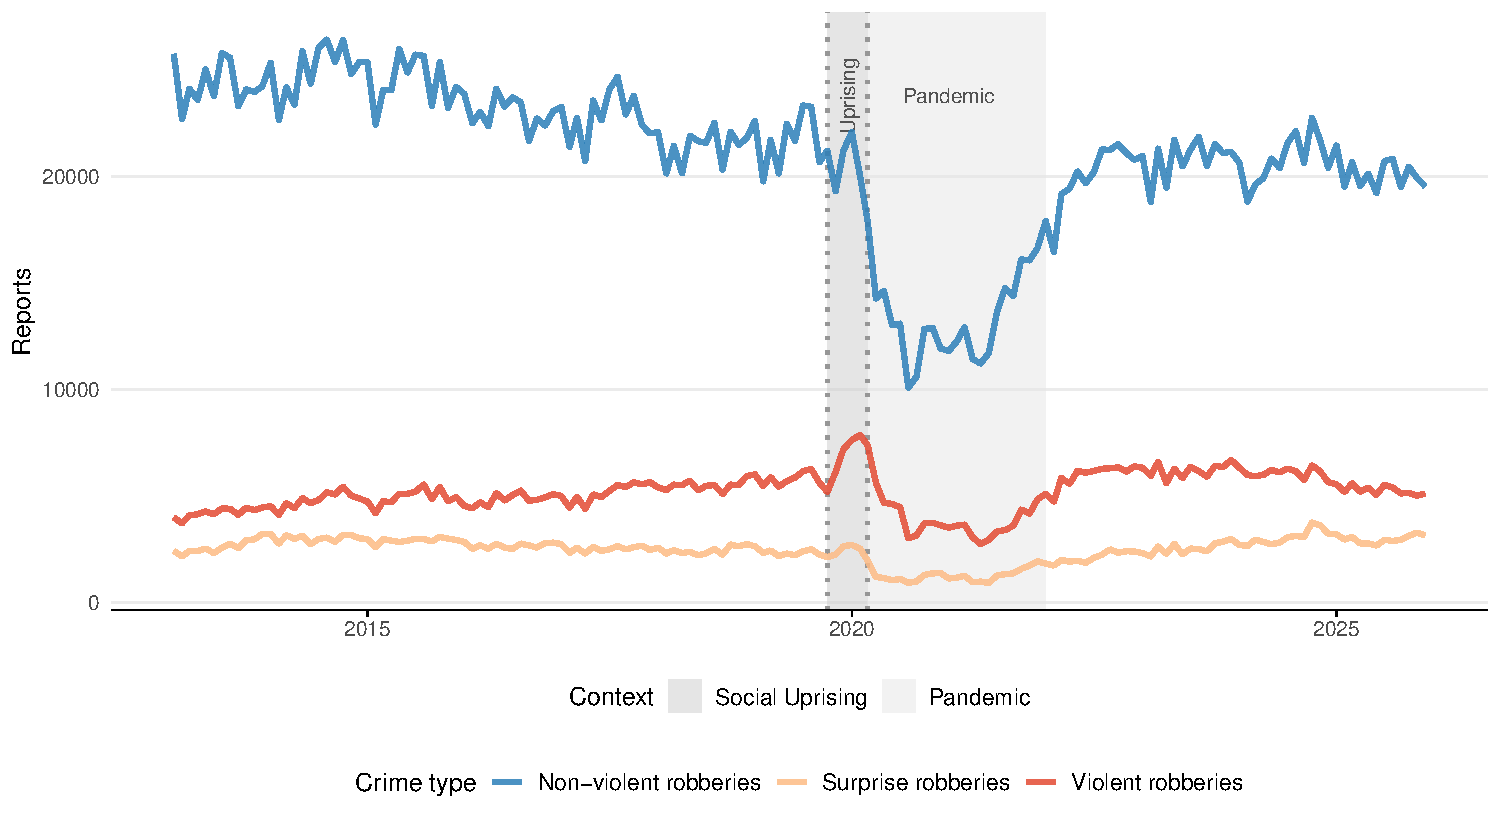
\includegraphics[width=\textwidth]{fig1_serie_mensual_nacional_eng.pdf}
\caption{Monthly series of police cases by C3 category, Chile 2013--2025.}
\label{fig:serie}
\tablenote{The shaded bands correspond to the social uprising (Oct.\ 2019--Feb.\
2020) and the pandemic (Mar.\ 2020--Dec.\ 2021). Rates per 100,000 inhabitants.
Source: \citet{INE2026}; INE Base 2024 projections (national level).}
\end{figure}

Annual rates reveal the structural pattern more clearly. Violent robberies
described an upward trajectory from 286 per 100,000
inhabitants in 2013 to 354 in 2019, collapsed to 206 during the pandemic (2021), and
recovered to reach a new peak of 343 in 2023 before initiating a downward inflection in 2024--2025 (283 in 2025). Importantly, after the historical peak of 2023, Spline~4 captures a downward trend that the model formalizes with IRR\,=\,0.868 ($p=0.057$), converging toward the levels at the start of the series. Non-violent robberies
show a secular decline spanning the entire period: from about 1,657
per 100,000 in 2013 to 1,130 in 2024, without significant post-pandemic
recovery. This divergence in trajectories---violent robberies with a new downward inflection, non-violent robberies in a pronounced and sustained decline---is the mechanism that generates
the paradox of the growing ratio (Figure~\ref{fig:tasas}).

\begin{figure}[htbp]
\centering
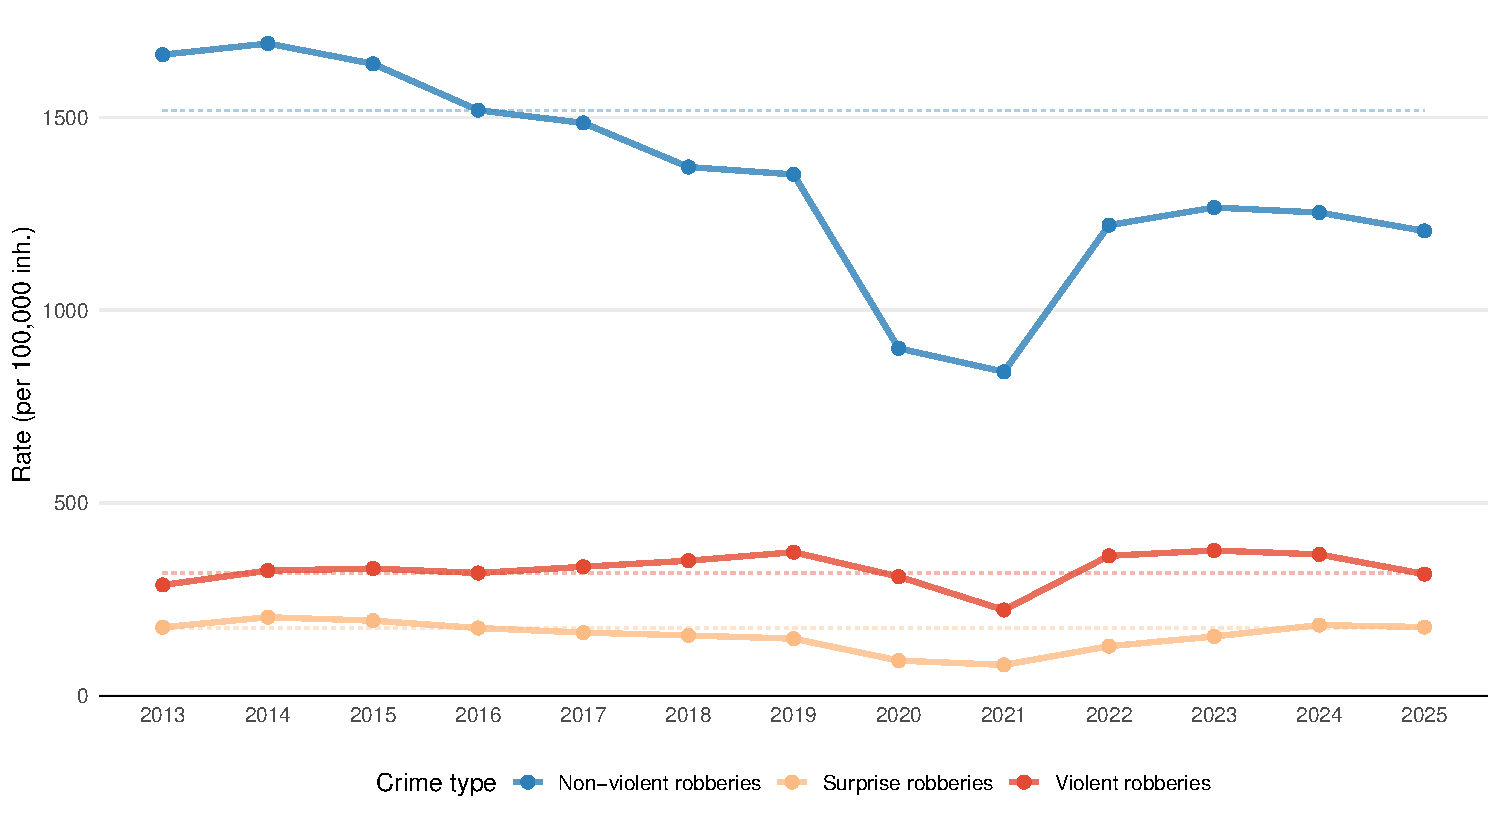
\includegraphics[width=\textwidth]{fig2_tasa_anual_nacional_eng.pdf}
\caption{Annual rates of police cases per 100,000 inhabitants, by C3 category,
Chile 2013--2025.}
\label{fig:tasas}
\tablenote{The horizontal reference lines correspond to the rate in 2016 for each
category. Source: \citet{INE2026}; INE Base 2024 projections (national level).}
\end{figure}

These divergences are quantified in Table~\ref{tab:descriptivo}, which synthesizes the descriptive statistics by period.

\begin{table}[htbp]
\centering
\caption{Descriptive statistics by period (violent robberies, regional panel)}
\label{tab:descriptivo}
\small
% \begin{adjustbox}{max width=\columnwidth}
\begin{tabular}{lcccc}
\toprule
\textbf{Period} & \textbf{N months} & \textbf{Mean} & \textbf{SD} & \textbf{Mean rate} \\
 & & (count) & (count) & (per 100,000) \\
\midrule
Pre-baseline (2013--2015)       & 36 & 290.3 & 719.5 & 15.5 \\
Baseline (2016--Sep.\ 2019)     & 45 & 330.0 & 875.2 & 14.9 \\
Uprising (Oct.\ 2019--Feb.\ 2020)  &  5 & 424.7 & 1200.8 & 17.4 \\
Pandemic (Mar.\ 2020--Dec.\ 2021)   & 22 & 247.2 & 698.4 & 10.3 \\
Post-pandemic (2022--2025)          & 48 & 366.6 & 939.1 & 16.3 \\
\bottomrule
\end{tabular}
% \end{adjustbox}
\tablenote{Observations: panel of 16 regions $\times$ number of months indicated.
The mean rate is the average across the 16 regions. Source: \citet{INE2026};
SERMIG; INE Base 2017 projections.}
\end{table}

Disaggregating the empirical data (Table~\ref{tab:cum}), the two crimes that dominate violent
robberies---robbery with intimidation (64.3\% of the group) and robbery with
violence (28.7\%)---record post-pandemic rates $-22.9\%$ and $-8.3\%$ below their
baseline period, respectively. Together they represent 93\% of the group
and their downward trend is the most robust element of the descriptive analysis.
Vehicle theft with violence (portonazo) appears in the system with substantial volume only since 2020,
representing 6.6\% of the group over the full period; therefore, its comparison takes 2020--2021 as a natural reference
baseline. The only crime with
sustained real growth is express kidnapping (retention of victims for ransom or extraction),
with an increase of 263\% between periods---but from a very low base (less
than 0.1\% of the group): 83 cases in 2022 versus 283 in 2025. In non-violent robberies,
the decline is generalized: the most pronounced corresponds to robbery in an inhabited place
($-35.0\%$) and theft of 0.5 to 4 UTM ($-25.7\%$).

\begin{table}[htbp]
\centering
\caption{Intra-category composition: main CUMs of the C3 classification (2013--2025)}
\label{tab:cum}
\footnotesize
% \begin{adjustbox}{max width=\columnwidth}
\begin{tabular}{lrp{5cm}rrrr}
\toprule
\textbf{Cat.} & \textbf{CUM} & \textbf{Description} & \textbf{Total N} & \textbf{\% group} & \textbf{Base rate\textsuperscript{a}} & \textbf{$\Delta$\%\textsuperscript{b}} \\
\midrule
\multicolumn{7}{l}{\textit{C3.1 --- Violent robberies}} \\
 & 802 & Robbery with intimidation        & 519,171 & 64.3 & 238.5 & $-$22.9 \\
 & 803 & Robbery with violence             & 232,073 & 28.7 &  97.7 & $-$8.3  \\
 & 867 & Vehicle theft w/viol. (portonazo) & 53,130 & 6.6 & --\textsuperscript{c} & n.a. \\
 & 828 & Robbery with rape           &   1,470 &  0.2 &  0.66 & $-$14.1 \\
 & 862 & Retention of victims      &     992 &  0.1 &  0.24 & $+$263  \\
 & 827 & Robbery with homicide             &     320 &  0.0 &  0.10 & $+$55   \\
 & 861 & Robbery with severe injuries       &     175 &  0.0 &  0.09 & $+$17   \\
 & 829 & Robbery w/castration/mutilation &   15  &  0.0 & 0.005 & $+$71   \\
\midrule
\multicolumn{7}{l}{\textit{C3.2 --- Surprise robberies}} \\
 & 804 & Surprise robbery (snatching)   & 382,445 & 100.0 & 158.2 & $-$8.0 \\
\midrule
\multicolumn{7}{l}{\textit{C3.3 --- Non-violent robberies}} \\
 & 808 & Robbery in public use place   & 739,657 & 22.7 & 317.3 & $-$18.9 \\
 & 809 & Robbery in inhabited place        & 589,940 & 18.1 & 268.9 & $-$35.0 \\
 & 847 & Theft 4--40 UTM               & 544,015 & 16.7 & 235.5 & $-$15.4 \\
 & 810 & Robbery in uninhabited place     & 480,777 & 14.7 & 206.6 & $-$15.8 \\
 & 848 & Theft 0.5--4 UTM              & 403,089 & 12.3 & 174.4 & $-$25.7 \\
 & 831 & Vehicle theft without viol.  & 350,990 & 10.8 & 137.0 & $-$4.8  \\
 & --- & Rest                          &    --- &  4.7 &   --- & variable \\
\bottomrule
\end{tabular}
% \end{adjustbox}
\tablenote{\textsuperscript{a} Average rate per 100,000 inh.\ in the baseline period
(2016--2019). \textsuperscript{b} Percentage change between base rate
(2016--2019) and post-pandemic rate (2022--2025). \textsuperscript{c} Portonazo is
activated in the system with significant volume since 2020; the base rate is not
comparable. Total N = police cases 2013--2025. Source: \citet{INE2026};
SERMIG; INE Base 2017 projections.}
\end{table}

The monthly ratio violent robberies/(violent + non-violent robberies), once seasonally adjusted
and smoothed using a local polynomial regression (LOESS; \textit{locally estimated
scatterplot smoothing}), rises almost monotonically from 14.7\% in April
2015 to an all-time high of 21.6\% in January 2024. The LOESS estimator fits
a weighted regression at each point on the closest temporal values;
the \texttt{span}\,=\,0.2 parameter is equivalent to using 20\% of the observations
as a smoothing window. Its function is exclusively descriptive: it reveals the
underlying trend filtered from short-term seasonal noise, without constituting a
formal hypothesis test; the resulting curve is consistent with---but conceptually
independent of---the formal Bai-Perron breaks. The Bai-Perron algorithm, selecting
$m=4$ breaks via BIC, identifies four successive inflections: Q1 in April 2015
(14.7\%), Q2 in August 2017 (17.1\%), Q3 in October 2019 (18.4\%), and Q4 in January
2024 (21.6\%). Each break marks a new ratio level, but the mechanism that
sustains them is not the growth of violent robberies, but the steeper contraction
of non-violent robberies in the denominator. This paradox---a growing ratio
alongside decreasing absolute volume---constitutes the central finding of the study
(Figure~\ref{fig:ratio}).

\begin{figure}[htbp]
\centering
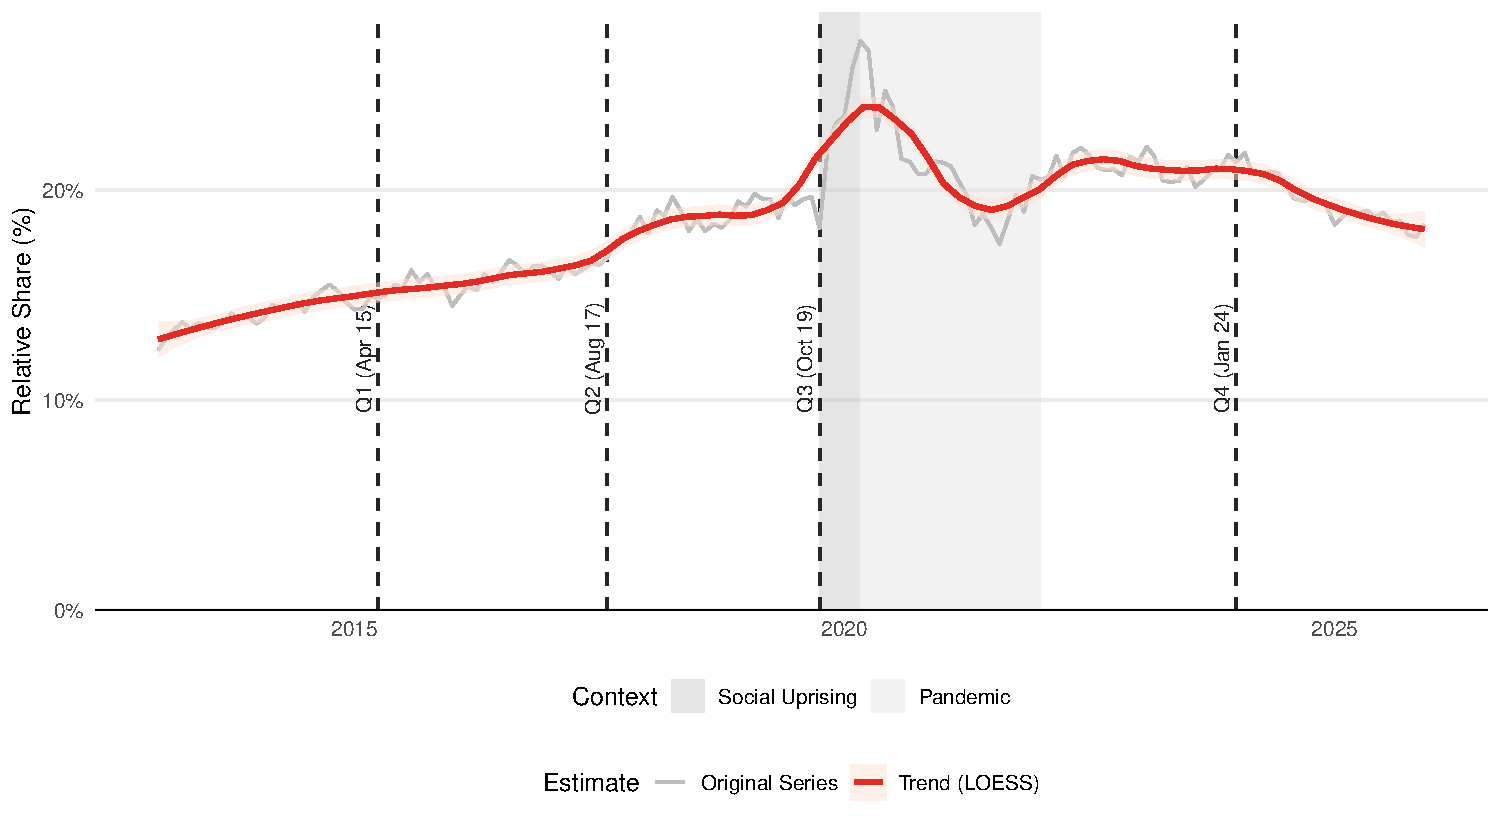
\includegraphics[width=\textwidth]{fig3_ratio_violentos_mensual_eng.pdf}
\caption{Monthly ratio violent robberies/(violent + non-violent robberies) with Bai-Perron breaks.}
\label{fig:ratio}
\tablenote{The dashed vertical lines mark the four optimal breaks by
BIC: Q1 = Apr.\ 2015 (14.7\%); Q2 = Aug.\ 2017 (17.1\%); Q3 = Oct.\ 2019 (18.4\%);
Q4 = Jan.\ 2024 (21.6\%). The series is seasonally adjusted. Source: \citet{INE2026}.}
\end{figure}

\subsection{Estimation of the secular trend}
\label{sub:inferencial}

Table~\ref{tab:poisson} reports the results of the Poisson-QMLE model for the
three C3 categories. For violent robberies, the social uprising produced a transient
increase of 15.5\% (IRR\,=\,1.155; $p<0.001$), consistent with the hypothesis that
the climate of protest facilitated direct-confrontation crimes. Surprise robberies
increased by 6.9\% (IRR\,=\,1.069; $p<0.001$). In contrast, non-violent robberies
did not react to the uprising (IRR\,=\,0.996; $p=0.761$): their dynamics
respond to structural opportunity factors, not to social conflict. The
pandemic produced a generalized and significant drop: $-34.9\%$ in violent ones
(IRR\,=\,0.651), $-42.4\%$ in surprise (IRR\,=\,0.576), and $-35.3\%$ in non-violent ones
(IRR\,=\,0.647). The greater intensity of the drop for surprise robberies reflects its dependence
on urban agglomeration, blocked by quarantines.

The most informative component is the spline's trajectory. For violent robberies,
the first three segments show moderate growth---Spline~1 (2013--2016):
IRR\,=\,1.178, $p=0.201$; Spline~2 (2016--2019): IRR\,=\,1.136, $p=0.087$;
Spline~3 (2019--2022): IRR\,=\,1.187, $p<0.001$. The most relevant result is
Spline~4, which captures the September 2022--December 2025 period: IRR\,=\,0.868
($p=0.057$ via WCB), indicating a downward inflection that begins to emerge
statistically. With $G=16$ clusters, a p-value of 0.057 is suggestive evidence;
its consistency with the descriptive analysis and placebos strengthens the
interpretation of a real decline.

For non-violent robberies, the decline is robust, monotonic, and significant across all
segments: all four spline coefficients are negative and highly significant,
with Spline~4 showing IRR\,=\,0.648 ($p<0.001$), a reduction of 35.2\% from
the initial level. This trend began before the pandemic and deepened throughout
the entire observed horizon, consistent with structural changes in
routine activities---retail e-commerce expansion and residential security.
For surprise robberies, secular decline dominates the initial segments
(Spline~1: IRR\,=\,0.668; Spline~2: IRR\,=\,0.635), eventually stabilizing in the recent
period (Spline~4: IRR\,=\,0.861, $p=0.574$). The divergence between categories
confirms the value of the trichotomous classification: the three types of robbery follow
qualitatively different trajectories.

\begin{table}[htbp]
\centering
\caption{Poisson-QMLE model with Wild Cluster Bootstrap: main results (C3)}
\label{tab:poisson}
\footnotesize
% \begin{adjustbox}{max width=\columnwidth}
\begin{tabular}{l@{\hskip 3mm}ccc@{\hskip 4mm}ccc@{\hskip 4mm}ccc}
\toprule
 & \multicolumn{3}{c}{\textbf{Violent robberies}} & \multicolumn{3}{c}{\textbf{Surprise robberies}} & \multicolumn{3}{c}{\textbf{Non-violent}} \\
\cmidrule(lr){2-4}\cmidrule(lr){5-7}\cmidrule(lr){8-10}
\textbf{Term} & IRR & 95\% CI & $p$ & IRR & 95\% CI & $p$ & IRR & 95\% CI & $p$ \\
\midrule
$D^{\text{up}}$ & 1.155 & [1.119, 1.192] & $<$.001 & 1.069 & [1.031, 1.108] & $<$.001 & 0.996 & [0.971, 1.022] & .761 \\
$D^{\text{pan}}$ & 0.651 & [0.621, 0.682] & $<$.001 & 0.576 & [0.547, 0.606] & $<$.001 & 0.647 & [0.628, 0.665] & $<$.001 \\
\midrule
Spline 1    & 1.178 & [0.917, 1.513] & .201 & 0.668 & [0.619, 0.722] & $<$.001 & 0.718 & [0.673, 0.767] & $<$.001 \\
Spline 2    & 1.136 & [0.982, 1.315] & .087 & 0.635 & [0.462, 0.873] & .005 & 0.685 & [0.568, 0.826] & $<$.001 \\
Spline 3    & 1.187 & [1.116, 1.264] & $<$.001 & 0.968 & [0.634, 1.480] & .882 & 0.656 & [0.570, 0.754] & $<$.001 \\
\textbf{Spline 4} & \textbf{0.868} & \textbf{[0.751, 1.004]} & \textbf{.057} & 0.861 & [0.511, 1.450] & .574 & \textbf{0.648} & \textbf{[0.580, 0.723]} & $<$.001 \\
\midrule
Obs. & 2,496 & & & 2,496 & & & 2,496 & & \\
\bottomrule
\end{tabular}
% \end{adjustbox}
\tablenote{IRR = exp($\hat{\beta}$). 95\% CI via WCB inversion (Webb weights,
$B=9,999$, $G=16$). $D^{\text{up}}$: social uprising dummy (Oct.\ 2019--Feb.\
2020). $D^{\text{pan}}$: pandemic dummy (Mar.\ 2020--Dec.\ 2021). Spline~1--4: restricted
cubic spline with knots at P25 ($\approx$ Mar.\ 2016), P50 ($\approx$ Jun.\ 2019),
and P75 ($\approx$ Sep.\ 2022). All models include regional fixed effects and
monthly seasonality dummies. Offset: $\log$(corrected monthly population).}
\end{table}

\subsection{Regional heterogeneity and CUSUM breaks}
\label{sub:regional}

The CUSUM-GLM tests reveal that the structural change in violent robberies is real but
temporally heterogeneous: 12 out of 16 regions present a significant break
(p-FDR\,<\,0.05), but at three different points in time responding to different local
logics (Table~\ref{tab:cusum}).

The first group, with pre-pandemic breaks, comprises regions of the South macro-zone
(Maule: April 2017; Biob\'io: August 2018; La Araucan\'ia: July 2018) and Magallanes
(August 2017). These inflections precede the social uprising by more than two years,
indicating local processes independent of the national shock: internal migration dynamics,
expansion of territorial illicit economies, and the reconfiguration of criminal networks in the south.
The second group, with breaks during the pandemic and reactivation, groups most regions---Metropolitan
Region (July 2020), Atacama (August 2021), O'Higgins (September 2021), Coquimbo
(September 2021), Arica y Parinacota (July 2021), and \~Nuble (August 2021)---with
inflections concentrated between July 2020 and September 2021. The combination of
mobility restrictions and subsequent reactivation reorganized criminal patterns
profoundly enough to generate statistically detectable breaks.
The third group, characterized by a late break, corresponds exclusively to Tarapac\'a (August 2023):
migration intensity from the northern border and the reconfiguration of organized crime routes explain this delay.
Four regions---Antofagasta, Valpara\'iso, Los Lagos, and Los R\'ios---show no
evidence of a significant break.

\begin{table}[htbp]
\centering
\caption{CUSUM-GLM tests: structural break in violent robberies by region}
\label{tab:cusum}
\footnotesize
% \begin{adjustbox}{max width=\columnwidth}
\begin{tabular}{llccc}
\toprule
\textbf{Region} & \textbf{Macro-zone} & \textbf{p-value} & \textbf{p-FDR} & \textbf{Estimated break} \\
\midrule
R15 --- Arica y Parinacota & North   & $<$.001  & $<$.001 & Jul.\ 2021 \\
R8 --- Biob\'io            & South     & $<$.001  & $<$.001 & Aug.\ 2018 \\
R9 --- La Araucan\'ia      & South     & $<$.001  & $<$.001 & Jul.\ 2018 \\
R7 --- Maule               & Central  & $<$.001  & $<$.001 & Apr.\ 2017 \\
R3 --- Atacama             & North   & $<$.001  & $<$.001 & Aug.\ 2021 \\
R6 --- O'Higgins           & Central  & $<$.001  & $<$.001 & Sep.\ 2021 \\
R13 --- Metropolitana      & MR      & $<$.001  & $<$.001 & Jul.\ 2020 \\
R11 --- Ays\'en            & Austral & .001     & .001    & Feb.\ 2016 \\
R12 --- Magallanes         & Austral & .001     & .003    & Aug.\ 2017 \\
R1 --- Tarapac\'a          & North   & .003     & .005    & Aug.\ 2023 \\
R4 --- Coquimbo            & North   & .006     & .009    & Sep.\ 2021 \\
R16 --- \~Nuble            & South     & .016     & .022    & Aug.\ 2021 \\
\midrule
R2 --- Antofagasta         & North   & .194     & .207    & (n.s.) \\
R5 --- Valpara\'iso        & Central  & .334     & .334    & (n.s.) \\
R10 --- Los Lagos          & South     & .176     & .201    & (n.s.) \\
R14 --- Los R\'ios         & South     & .144     & .177    & (n.s.) \\
\bottomrule
\end{tabular}
% \end{adjustbox}
\tablenote{Supremum Brownian bridge test on the empirical fluctuation process of the regional GLM.
p-FDR: Benjamini-Hochberg correction on the 16 p-values. The estimated break corresponds to the month of the highest accumulation of the CUSUM statistic.}
\end{table}

The cumulative trajectory of the residuals in each region shows how the process exceeds
the 95\% critical limits at different times, highlighting the absence of a synchronous
national shock (Figure~\ref{fig:cusum}). Geographically, pre-pandemic breaks are concentrated
in the south, while those of the pandemic and reactivation are distributed across
the center and north of the country (Figure~\ref{fig:mapatasa}).

\begin{figure}[htbp]
\centering
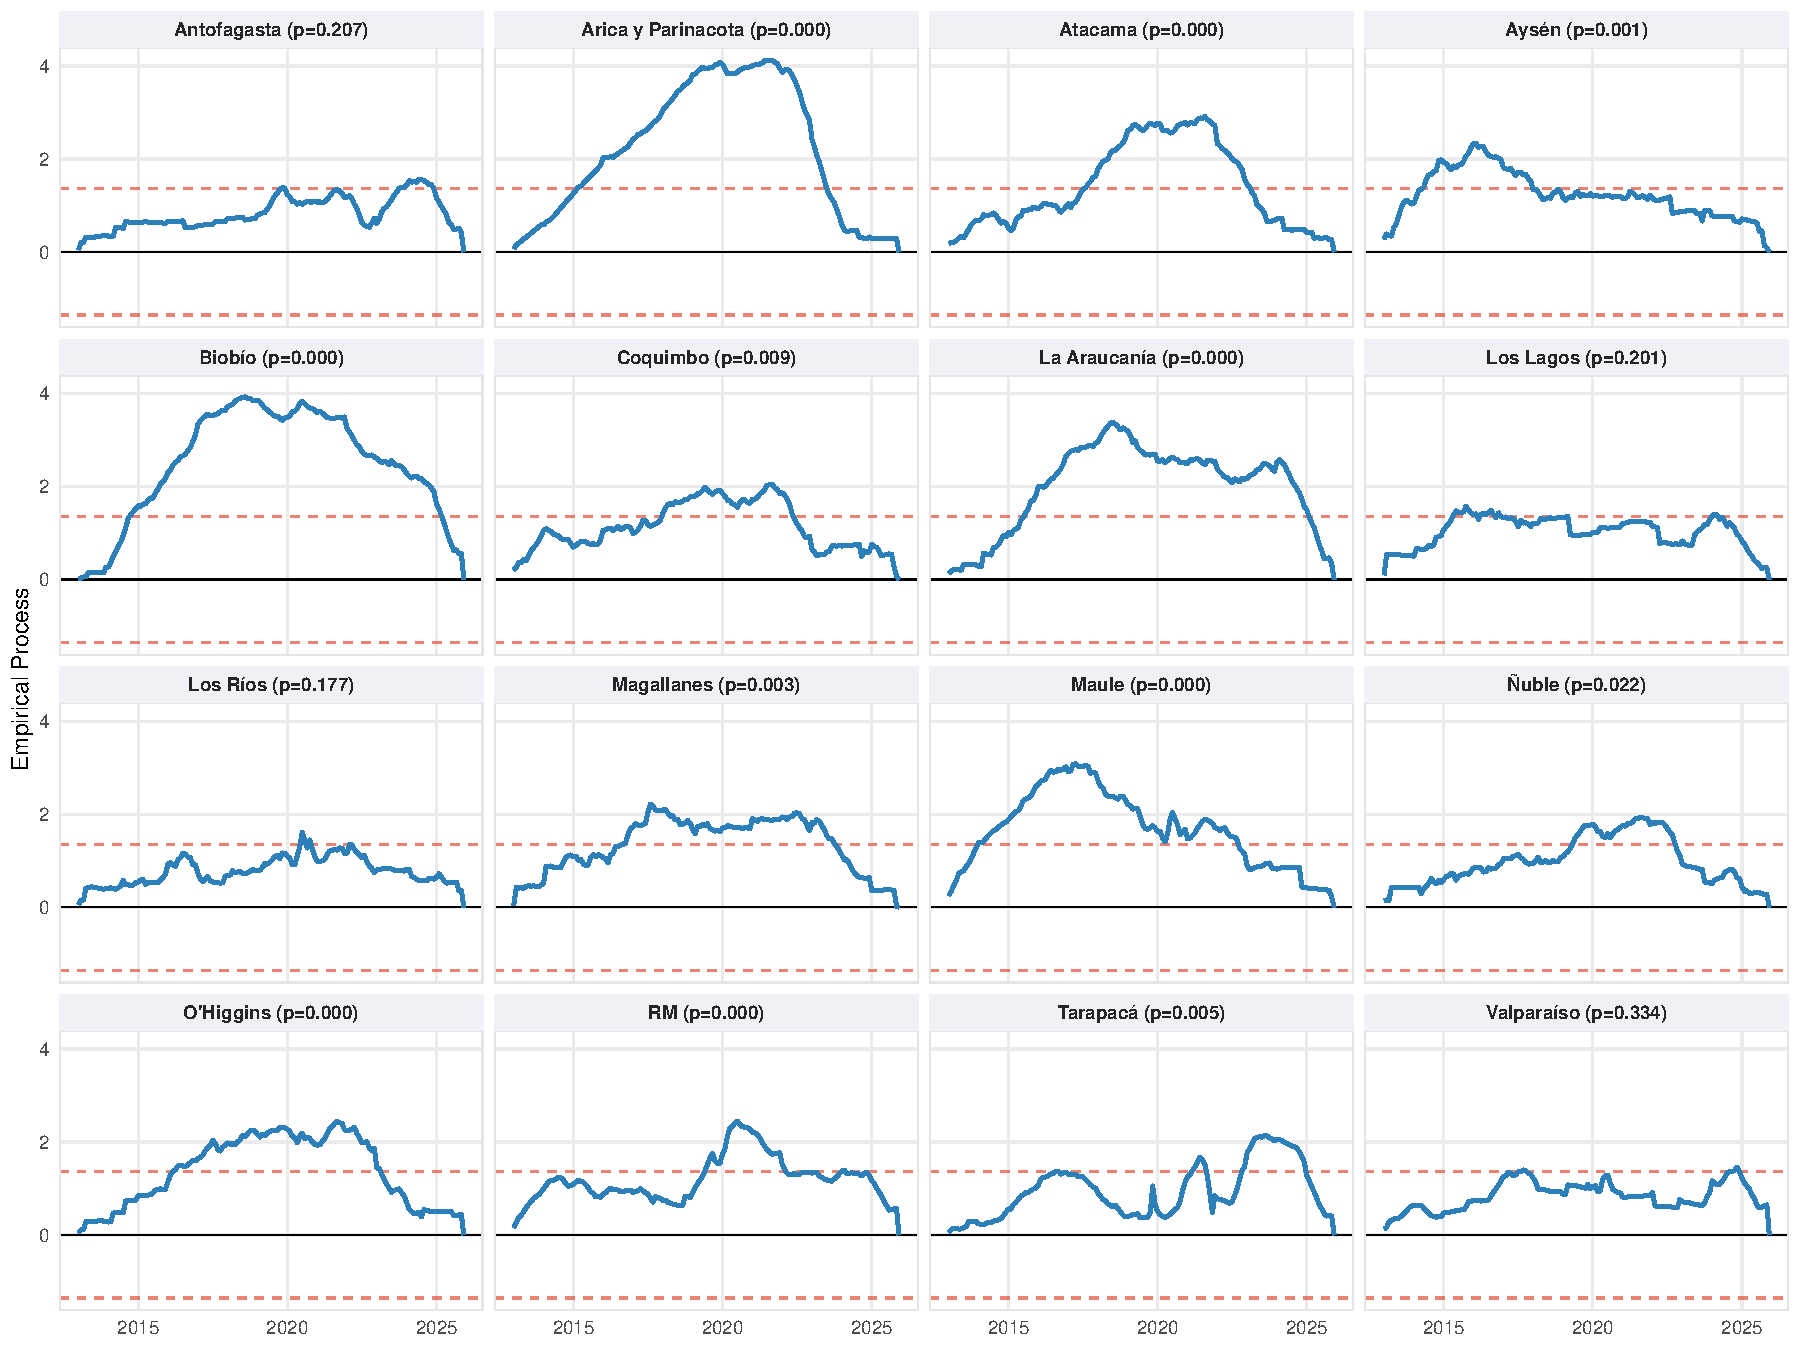
\includegraphics[width=\textwidth]{fig4_cusum_regional_facet_eng.pdf}
\caption{CUSUM-GLM processes for the 16 regions (violent robberies, C3.1).}
\label{fig:cusum}
\tablenote{The bands correspond to the 95\% critical limits of the Brownian bridge process.
Regions with a significant break (p-FDR\,<\,0.05) are highlighted in
red. Source: \citet{INE2026}; SERMIG; INE Base 2017 projections.}
\end{figure}
A direct comparison between Spline~1 (2013--2016) and Spline~4 (2022--2025) shows substantial regional heterogeneity in the violent robbery rate (Figure~\ref{fig:mapatasa}).
Northern regions, particularly Arica y Parinacota, exhibit the largest increases between the two periods, consistent with migratory pressure and the identified CUSUM breaks. Southern regions with early breaks tend to show more modest inter-period differences.

\begin{figure}[htbp]
\centering
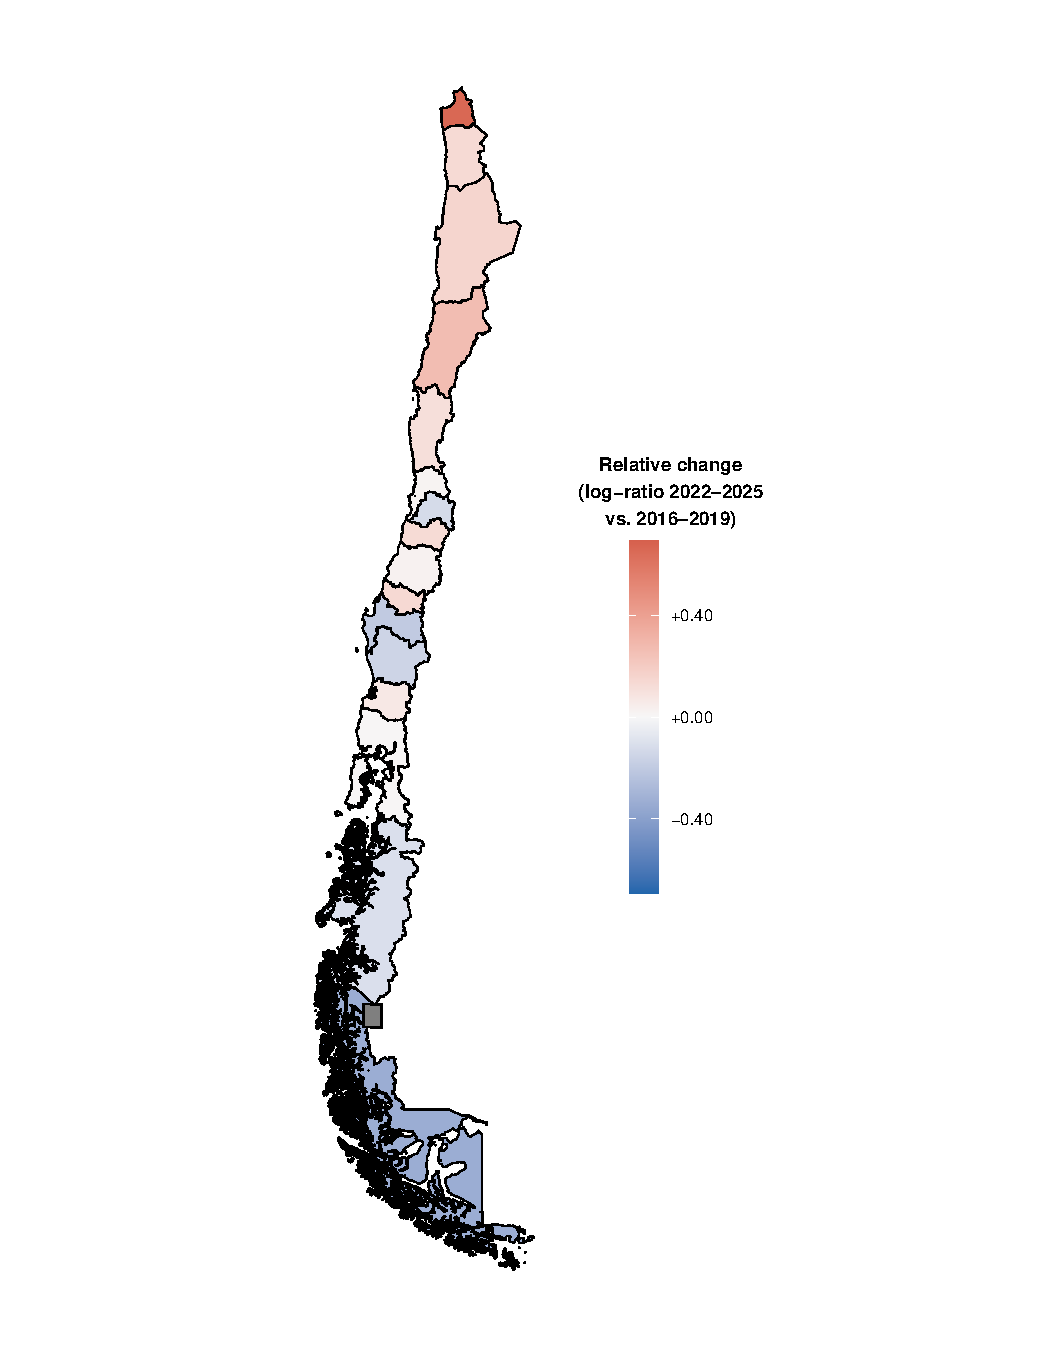
\includegraphics[width=0.88\textwidth]{map_logratio_regional_eng.pdf}
\caption{Rates of violent robberies by region: Spline~1 (2013--2016) versus Spline~4 (2022--2025), per 100,000 inh.}
\label{fig:mapatasa}
\tablenote{Period average in each region. Source: \citet{INE2026};
SERMIG; INE Base 2017 projections.}
\end{figure}

The macro-zone $\times$ spline interaction model (Appendix~\ref{ap:macro}) reveals that the long-term trend differs significantly between geographic zones (joint Wald test: $p<0.001$). In the first segment (Spline~1, 2013--2016), the Metropolitan Region exhibits the highest relative growth (IRR\,=\,2.68 with respect to Austral), followed by the Central macro-zone (IRR\,=\,1.82). In Spline~2 (2016--2019), the North macro-zone leads with the highest IRR (3.94), consistent with accumulated migratory pressure and the CUSUM break identified in Arica y Parinacota (July 2021, with a lag that suggests latent accumulation). In Spline~3 (2019--2022), the Center reaches its highest dynamism (IRR\,=\,3.57). In Spline~4 (2022--2025), however, all interactions converge toward unity---North: IRR\,=\,1.08; Central: 1.37; South: 1.00---indicating that the recent downward inflection is a phenomenon of national scope and not an artifact of any particular zone.

\subsection{Validation via placebos}
\label{sub:placebos}

Four validation models provide converging evidence regarding the specificity and
power of the primary model (Table~\ref{tab:placebos}).

The negative placebo (P1, vehicular quasi-crimes) reflects the reactivation of
driving activity post-pandemic: all its spline segments are positive and significant,
with Spline~4 showing IRR\,=\,2.036 ($p<0.001$). The same model that detected a
negative inflection in violent robberies captures a pronounced growth here. This
rules out the possibility that the specification systematically underestimates
activity in the most recent period: the negative result of Spline~4 in violent robberies
is not a model artifact.

The positive placebo (P2, CCH intentional homicides) offers the direct counterproof: if real violence
is increasing, the model must detect it. And so it does.
Splines~2 and 3 register IRR\,=\,2.746 and 3.612 ($p<0.001$ in both), capturing the
real increase in homicides between 2016 and 2022. In Spline~4, homicides
yield IRR\,=\,2.061 ($p<0.001$)---still in growth territory, unlike
violent robberies which show a downward inflection. This divergence between
homicides (growing in Spline~4) and violent robberies (decreasing) cannot be attributed
to a specification problem: the model differentially detects opposite dynamisms,
validating its discriminant capacity. Additionally, macro-zone level triangulation of homicides reveals that this lethal rise is neither spatially symmetric nor synchronous. While the Austral macro-zone exhibits no significant break in its series, the North macro-zone experienced the sharpest and earliest rise during the 2016--2019 period (Spline~2: IRR\,=\,2.25, $p<0.001$). In contrast, the Central, MR, and South macro-zones show a prolonged steady growth trajectory, achieving their highest relative expansion velocity between 2019 and 2022 (Spline~3 with IRR coefficients above 2.65). This indicates that, while violent robberies retreat nationally after the pandemic, the resurgence of lethality possessed differentiated regional moorings and chronologies.

A second positive placebo (P3, kidnappings) offers complementary validation. If
coercive organized crime expanded in the 2022--2025 period, the model must
register growth in kidnappings. Spline~4 for kidnappings yields
IRR\,=\,1.553 ($p<0.001$), the highest coefficient among all placebos in
the recent period. This result is consistent with the 263\% increase in the
retention of victims documented in Table~\ref{tab:cum} and reinforces the
interpretation that coercive organized crime indeed expanded in that
period. The coexistence of a downward inflection in total violent robberies
(IRR\,=\,0.868) with pronounced growth in kidnappings (IRR\,=\,1.553) confirms
that the model discriminates among different forms of property violence: the drop
in aggregate volume does not preclude detecting emerging highly harmful phenomena.

The triangulation with the CPHDV confirmed homicides provides the most robust reference
point against the dark figure. Annual records show a
growth from approximately 900 confirmed homicides in 2018 to a peak
of 1,330 in 2022, followed by a steady decline: 1,249 in 2023, 1,209 in 2024, and
1,091 in 2025. Spline~4 for CPHDV is not statistically significant
(IRR\,=\,1.075, $p=0.530$), indicating that the growth of lethal violence
decelerated in the most recent period. The parallel moderation in confirmed homicides
and violent robberies draws a coherent picture: both indicators point
to a ceiling reached around 2022 and subsequent deceleration.

\begin{table}[htbp]
\centering
\caption{Placebos and external validation: Poisson-QMLE models}
\label{tab:placebos}
\footnotesize
% \begin{adjustbox}{max width=\columnwidth}
\begin{tabular}{l@{\hskip 3mm}ccc@{\hskip 4mm}cc@{\hskip 4mm}cc@{\hskip 4mm}cc}
\toprule
 & \multicolumn{3}{c}{\textbf{P1: Vehicular accident}} & \multicolumn{2}{c}{\textbf{P2: CCH Homicides}} & \multicolumn{2}{c}{\textbf{P3: Kidnappings}} & \multicolumn{2}{c}{\textbf{CPHDV (confirmed)}} \\
\cmidrule(lr){2-4}\cmidrule(lr){5-6}\cmidrule(lr){7-8}\cmidrule(lr){9-10}
\textbf{Term} & IRR & 95\% CI & $p$ & IRR & $p$ & IRR & $p$ & IRR & $p$ \\
\midrule
$D^{\text{up}}$ & 1.105 & [0.989, 1.234] & .078 & 1.144 & .097 & 0.869 & .146 & 1.046 & .763 \\
$D^{\text{pan}}$ & 0.874 & [0.750, 1.020] & .087 & 1.009 & .949 & 0.572 & $<$.001 & 0.871 & .367 \\
\midrule
Spline 1 &  9.080 & [3.09, 26.70] & $<$.001 & 1.300 & .096 & 1.338 & .024 & 1.562 & .001 \\
Spline 2 &  3.820 & [1.85,  7.90] & $<$.001 & 2.746 & $<$.001 & 2.654 & $<$.001 & 1.430 & $<$.001 \\
Spline 3 & 48.380 & [6.78, 345.4] & $<$.001 & 3.612 & $<$.001 & 1.649 & .024 & 1.774 & .113 \\
\textbf{Spline 4} & \textbf{2.036} & [1.397, 2.969] & $<$.001 & \textbf{2.061} & $<$.001 & \textbf{1.553} & $<$.001 & 1.075 & .530 \\
\bottomrule
\end{tabular}
% \end{adjustbox}
\tablenote{P1, P2, and P3 are estimated on the regional panel (16 regions $\times$ 156 months);
CPHDV on the national series (2018--2025, native knots). The large IRRs of P1 in
Spline~3 reflect the normalization of post-pandemic traffic on a logarithmic scale.
Inference: WCB (Webb weights, $B=9,999$) for P1, P2, and P3; standard QMLE errors
for CPHDV.}
\end{table}




% =========================================================
\section{Robustness analysis}
\label{sec:robustez}
% =========================================================

The robustness analysis examines the stability of the main result under six dimensions of
variation. Dimensions R1, R3, and R5 evaluate sensitivity to the denominator and trend
parametrization; R6 replaces reports with arrests in flagrancy to explore the dissociation
between citizen victimization and police activity; R7 adds flexibility to the spline;
and the dichotomous classifications C1 and C2---reported in Appendix~\ref{ap:clasif}---constitute an additional dimension of classification sensitivity.

Table~\ref{tab:robustez} reports the Spline~4 coefficient (2022--2025) under six
alternative specifications for violent robberies. Five of the six specifications
produce negative coefficients, confirming the downward inflection of the main
model (IRR\,=\,0.868, $p=0.057$). Specifications R1 (free offset:
IRR\,=\,0.732, $p=0.010$) and R6 (arrests in flagrancy: IRR\,=\,0.539, $p<0.001$)
produce declines even steeper than the baseline model; R5 (theoretical knots:
IRR\,=\,0.883, $p=0.079$) and R7 (more flexible spline, df\,=\,5: IRR\,=\,0.863,
$p=0.068$) replicate the magnitude of the main finding with practically identical coefficients.

Specification R3 (without the SERMIG correction) is the only exception:
it produces a practically null coefficient (IRR\,=\,0.994, $p=0.948$). The exclusion
of the migratory correction introduces noise in the denominator of high-immigration
regions, attenuating the signal to zero; this result illustrates the
empirical relevance of the SERMIG correction and does not contradict the direction
of the main finding. Specification R6, whose coefficient is the most negative,
indicates that arrests in flagrancy during the 2022--2025 period fell even
more intensely than reported police cases, which rules out the possibility that the
downward inflection is an artifact of the dark figure or changes in the propensity
to report.

\begin{table}[htbp]
\centering
\caption{Robustness analysis: trend coefficient under alternative specifications
(violent robberies, C3.1)}
\label{tab:robustez}
\small
% \begin{adjustbox}{max width=\columnwidth}
\begin{tabular}{llccc}
\toprule
\textbf{ID} & \textbf{Specification} & \textbf{Estimator} & \textbf{IRR} & $p$ \\
\midrule
Main & Baseline model (spline P25/P50/P75, WCB) & $-$0.141 & 0.868 & .057 \\
\midrule
R1 & Free offset (pop.\ as regressor)      & $-$0.312 & 0.732 & .010 \\
R3 & Without SERMIG correction             & $-$0.006 & 0.994 & .948 \\
R5 & Theoretical knots (2016, 2019, 2022)  & $-$0.125 & 0.883 & .079 \\
R6 & Arrests as dependent variable         & $-$0.618 & 0.539 & $<$.001 \\
R7 & More flexible spline (df\,=\,5)       & $-$0.147 & 0.863 & .068 \\
\bottomrule
\end{tabular}
% \end{adjustbox}
\tablenote{The reported estimator corresponds to Spline~4 of the model (trend in the
2022--2025 period), which is the main term of interest. All
specifications include uprising/pandemic dummies, regional fixed effects, and
monthly seasonality.}
\end{table}

Table~\ref{tab:sensipop} examines the sensitivity to the irregular population denominator
under demographic inflation factors $k \in \{1.00, 1.05, 1.10, 1.15, 1.20\}$ applied to high-immigration regions. The Spline~4 estimator and IRR
remain identical across all scenarios (estimator\,=\,$-0.141$; IRR\,=\,0.868),
with minimal variations in the standard error that do not alter inference (p-value
range: 0.048--0.062). The
invariance is explained because the factor $k$ shifts the offset uniformly, affecting
the intercept but not the trend coefficients. The results are therefore robust
to any plausible assumption about the irregular population not captured by SERMIG.

\begin{table}[htbp]
\centering
\caption{Sensitivity to the irregular denominator: inflation factor $k$ on
corrected population (violent robberies)}
\label{tab:sensipop}
\small
% \begin{adjustbox}{max width=\columnwidth}
\begin{tabular}{ccccc}
\toprule
\textbf{Factor $k$} & \textbf{Estimator} & \textbf{SE (WCB)} & \textbf{IRR} & $p$ \\
\midrule
1.00 & $-$0.141 & 0.071 & 0.868 & .048 \\
1.05 & $-$0.141 & 0.075 & 0.868 & .061 \\
1.10 & $-$0.141 & 0.074 & 0.868 & .057 \\
1.15 & $-$0.141 & 0.072 & 0.868 & .050 \\
1.20 & $-$0.141 & 0.076 & 0.868 & .062 \\
\bottomrule
\end{tabular}
% \end{adjustbox}
\tablenote{$k$ = inflation factor applied to the corrected population of high-immigration
regions (Tarapac\'a, Antofagasta, Arica y Parinacota, Metropolitan Region). The invariance of the estimator and IRR confirms that the results are
independent of assumptions about the irregular population.}
\end{table}


% =========================================================
\section{Discussion}
\label{sec:discusion}
% =========================================================

The evidence presented suggests that the public debate over the ``security crisis''
in Chile captures something real, but describes it inaccurately. What exists is a
qualitative shift in the composition of property crime: today a larger
fraction of robberies involves direct confrontation with the victim, even though the
absolute number of those robberies is lower than in 2019. This compositional shift is
statistically robust---the ratio of violent robberies to total robberies reached a historical
maximum of 21.6\% in January 2024, confirmed by four successive
Bai-Perron breaks and by the spline divergence between categories---but its mechanism
is the accelerating decline of non-violent robberies, not an increase in
violent robberies.

The logic of the mechanism is plausible from the perspective of routine activity theory.
The expansion of e-commerce and home delivery platforms
reduces the circulation of physical goods in public spaces. Heightened residential
security---proliferation of fences, cameras, and alarms---reduces the profitability of
robbery in homes and uninhabited spaces. Crimes requiring direct coercion
are less sensitive to these barriers: the offender who uses intimidation or violence
confronts the victim directly and does not depend on absence or vulnerability conditions. The
result is that robberies without confrontation disappear faster than those
that require it, raising the ratio even as the total volume falls.

Despite the general picture of stabilization in the volume of violent robberies, two
emerging phenomena demand attention. The first is victim retention:
although it represents less than 0.1\% of the group, it grew by 263\% between the
compared periods, rising from 83 cases in 2022 to 283 in 2025. This phenomenon answers to
an organized crime logic---coercion for bank transfers---that
demands differentiated policy responses. The second is the level of intentional
homicides: despite the decline post-2022, the 1,091 confirmed homicides in 2025
remain substantially above the levels prior to the social uprising.

In this context, the territorial trajectory of organized crime in the North macro-zone
reveals a biphasic structure that is remarkably captured by the inferential and validation models.
While the increase in lethal violence (intentional homicides) presented its most
expansive and earliest phase there during the 2016--2019 period (IRR\,=\,2.25), the overflow
of violence specifically oriented toward property coercion (violent robberies)
only registered its structural breaks in this macro-zone around 2021--2023. This
chronological dissociation suggests that the initial installation of criminal networks operated
through lethal territorial control in a first phase, only to evolve into a
second phase of extractive maturation over citizens' property post-pandemic.

The distinction between volume and composition has direct consequences for policy
design. A volume-based response---more police presence to reduce
the total number of incidents---is misdirected if the dynamic is compositional. The
evidence suggests that interventions must be targeted toward emerging phenomena
of high severity: strategies for protecting banking and digital payment channels
against express kidnappings, and the sustained dismantling of organized crime
structures linked to lethal violence.

Four limitations should be considered. The effect of Comisaria Virtual on the
reporting propensity cannot be directly controlled, given that the CCH records
do not identify the reporting channel. Vehicle theft with violence (portonazo) activates with significant volume
only starting in 2020, limiting the comparable history of this code. The small
number of clusters ($G=16$) means the Spline~4 p-value for violent robberies
($p=0.057$) should be interpreted with caution, although its consistency with the placebos
and the descriptive analysis mitigates this limitation. Finally, the SERMIG correction
is a lower bound of the true population; the sensitivity analysis demonstrates
coefficient invariance under different assumptions for the irregular population.


% =========================================================
\section{Conclusions}
\label{sec:conclusiones}
% =========================================================

This article provides systematic empirical evidence for the debate on
property crime in Chile during the 2013--2025 period. The main
findings are fourfold.

First, the aggregate rate of violent robberies increased relative to Spline~1
(2013--2016), reached a historical peak in 2023, and initiated a downward
inflection formalized in Spline~4 (IRR\,=\,0.868, $p=0.057$), which is
suggestive although at the borderline of conventional significance. The rise in the total rate between 2020 and 2023 reflects in part the
emergence of vehicle theft with violence or intimidation, a crime whose volume
in the system became significant only starting that year and whose trajectory merits
independent monitoring.

Second, the ratio of violent robberies to total property crime reached a historical
maximum (21.6\% in January 2024) via a compositional mechanism: non-violent
robberies structurally declined faster than violent ones (Spline~4 non-violent:
IRR\,=\,0.648, $p<0.001$). The change is qualitative, not quantitative.

Third, the regional structural break is real but heterogeneous: 12 out of 16 regions
present a significant CUSUM break at three distinct points in time. There is no
single synchronous national shock.

Fourth, genuine emerging signals are identified: the sustained growth of
victim retention (+263\% between periods) and the level of intentional
homicides, which peaked in 2022 and, despite declining, remains above the
pre-uprising period.

It is not possible to respond to a qualitative change in the composition of crime with the
same tools that would be used to address a volumetric increase. The focus
must be on emerging highly harmful phenomena and on the organized
crime structures that sustain them.

% =========================================================
%  REFERENCES
% =========================================================
\newpage
\bibliography{../referencias}


% =========================================================
%  APPENDICES
% =========================================================
\newpage
\appendix

\section{Classification sensitivity: results under C1 and C2}
\label{ap:clasif}

Classification C1 (institutional binary) includes surprise robbery
in the ``violent'' category, following the official convention. This dilutes the
signal of the spline: the dynamics of snatching---strongly sensitive to the mobility
cycle---mix with those of high-harm robberies, attenuating the trend
coefficients toward non-significance across all segments. Classification C2 excludes
fencing (receptaci\'on) but maintains the binary grouping, with results that converge
with those of the violent C3 model (Table~\ref{tab:clasif}).

\begin{table}[htbp]
\centering
\caption{Comparison of Poisson-QMLE results according to binary classification}
\label{tab:clasif}
\footnotesize
% \begin{adjustbox}{max width=\columnwidth}
\begin{tabular}{l@{\hskip 3mm}ccc@{\hskip 4mm}ccc}
\toprule
 & \multicolumn{3}{c}{\textbf{C1 (official classification)}} &
   \multicolumn{3}{c}{\textbf{C2 (without fencing)}} \\
\cmidrule(lr){2-4}\cmidrule(lr){5-7}
\textbf{Term} & IRR & 95\% CI & $p$ & IRR & 95\% CI & $p$ \\
\midrule
$D^{\text{up}}$ & 1.132 & [1.097, 1.168] & $<$.001 & 1.155 & [1.119, 1.192] & $<$.001 \\
$D^{\text{pan}}$ & 0.634 & [0.609, 0.660] & $<$.001 & 0.651 & [0.622, 0.682] & $<$.001 \\
\midrule
Spline 1 & 0.974 & [0.797, 1.190] & .795 & 1.178 & [0.916, 1.514] & .202 \\
Spline 2 & 0.938 & [0.867, 1.014] & .107 & 1.136 & [0.981, 1.316] & .089 \\
Spline 3 & 1.094 & [0.936, 1.278] & .257 & 1.187 & [1.116, 1.263] & $<$.001 \\
\textbf{Spline 4} & 0.864 & [0.652, 1.145] & .308 & \textbf{0.868} & [0.751, 1.004] & \textbf{.057} \\
\midrule
Obs. & 2,496 & & & 2,496 & & \\
\bottomrule
\end{tabular}
% \end{adjustbox}
\tablenote{IRR = exp($\hat{\beta}$). 95\% CI via WCB inversion ($B=9,999$,
$G=16$). C1 includes surprise robbery in the ``violent'' category. C2 excludes fencing (receptaci\'on).
The results of C2 are equivalent to those of the C3.1 model in
Table~\ref{tab:poisson}. The loss of significance in all splines under C1
reflects the attenuation produced by including snatching.}
\end{table}

\section{Spatial heterogeneity: macro-zone $\times$ spline coefficients}
\label{ap:macro}

The interaction model estimates coefficients for each spline segment in each
macro-zone, using the Austral Macro-zone as a reference. The interaction IRRs
are interpreted as the multiplicative factor adjusting the trend of each macro-zone
with respect to Austral in that period: an IRR greater than 1 indicates that the macro-zone grows
(or falls less) faster than Austral (Table~\ref{tab:macro}).

\begin{table}[htbp]
\centering
\caption{IRRs of macro-zone $\times$ spline interactions (reference: Austral)}
\label{tab:macro}
\small
% \begin{adjustbox}{max width=\columnwidth}
\begin{tabular}{lcccc}
\toprule
\textbf{Macro-zone} & \textbf{Spline 1} & \textbf{Spline 2} & \textbf{Spline 3} & \textbf{Spline 4} \\
 & (2013--2016) & (2016--2019) & (2019--2022) & (2022--2025) \\
\midrule
North   & 1.41 & 3.94 & 3.25 & 1.08 \\
Central  & 1.82 & 2.63 & 3.57 & 1.37 \\
MR      & 2.68 & 2.22 & 3.03 & 1.46 \\
South     & 1.49 & 2.14 & 2.88 & 1.00 \\
Austral & ref. & ref. & ref. & ref. \\
\midrule
\multicolumn{5}{l}{Joint Wald test (interactions): $p < 0.001$} \\
\bottomrule
\end{tabular}
% \end{adjustbox}
\tablenote{IRR = exp($\hat{\beta}_{\text{interaction}}$). North: R15, R1, R2, R3, R4;
Central: R5, R6, R7; Metropolitan Region (MR): R13; South: R8, R9, R14, R16, R10; Austral: R11, R12.
Heterogeneity is most pronounced in Splines~2 and 3, especially for North and
MR. In Spline~4, all interactions approach 1 (North: 1.08; South: 1.00),
indicating that the recent downward inflection is national in scope. Source:
\citet{INE2026}; SERMIG; INE Base 2017 projections.}
\end{table}

% =========================================================
\end{document}
% =========================================================
